% Section content template for individual Educative lessons
% This file contains the actual content for a specific section
% Generated from Educative API section content

% Section: Introduction to Object-oriented Analysis and Design (OOAD)
% Section ID: 5399405387841536
% Section Slug: introduction-to-object-oriented-analysis-and-design-ooad
% Generated: 2025-12-08T22:20:39.579418

\subsection{OOAD in the SDLC}\label{8j59raf_4ZAEY05hB1Hgk}
\\
The \textbf{Software Development Life Cycle (SDLC)} refers to the sequence of phases involved in software development. The stages of SDLC are shown below.

\begin{figure}[htbp]
 \centering
 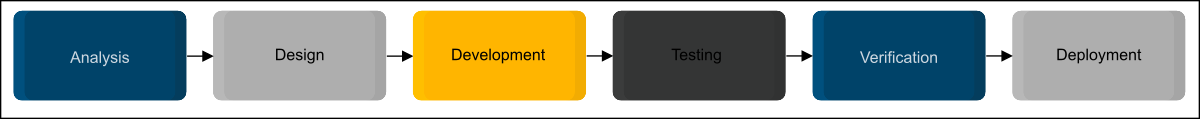
\includegraphics[width=0.5\textwidth]{Images/chapter_3/section_5399405387841536/5640597640839168.png}
 \caption{Stages of SDLC}
\end{figure}

The object-oriented analysis and design (OOAD) in SDLC allows one to analyze and design a system using object-oriented concepts and visualize each aspect of the OOAD process. In OOAD, we examine and inspect the entire system required for a particular problem, followed by identifying what it refers to as ``objects'' present in the system. It then establishes a relationship between the different objects and works on modeling and building a design for the whole system. This entire process is summarized in the following diagram:

\begin{figure}[htbp]
 \centering
 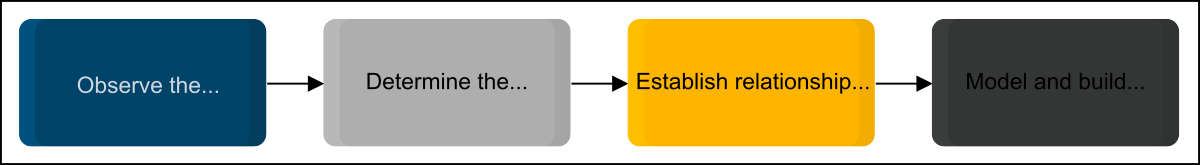
\includegraphics[width=0.5\textwidth]{Images/chapter_3/section_5399405387841536/5530061853949952.png}
 \caption{Object-oriented analysis and design process}
\end{figure}

Let's now explore the analysis and design stages of the OOAD process in further detail.

\subsection{Object-oriented analysis}\label{aRxOjKJjEtPVwgMl5GJnm}
\\
Object-oriented analysis is a method used to identify system requirements. This method creates a model by defining the roles of the objects in the system. It also defines the tasks for which the system is responsible. The analysis step excludes any implementation details. Instead , we focus on identifying different use cases.

\subsection{Object-oriented design}\label{2urde7A2qREP835oC2yU_}
\\
Object-oriented design is the phase where the implementation of the defined requirements and the models created during the analysis phase begins. In this step, the models are further refined by adding additional constraints and making decisions such as adding new elements to the given initial structure. At this stage, the designer also goes into the inner details of the defined models and elaborates if any object-oriented principle is required. These models are usually built using Unified Modeling Language (UML) diagrams such as class or sequence diagrams which will be explained in detail in this chapter.

\subsection{Advantages of OOAD}\label{wu__3ToJNcNkZC9D9pvOS}
\\
The object-oriented analysis and design process is highly well-known. The following are a few reasons why it is quite renowned among the community:

\begin{itemize}
\item
\protect\phantomsection\label{uKb8-15dgGBYj1Jjtz0mY}
It's extremely easy to understand, which helps in creating models of complex problems.
\item
\protect\phantomsection\label{uinFTVPUVApS7b595BZBN}
Concepts such as inheritance help make the data reusable and scalable.
\item
\protect\phantomsection\label{FrA0CX46aIqg0dda9Mlkt}
It's easily maintainable, which helps identify the issues in the early processes and saves time.
\end{itemize}
\\
Let's look at the Unified Modeling Language (UML) in the next lesson.

% End of section content